%\section{Introducción}

%%%%%%%%%%%%%%%%%%%%%%%%%%%%%%%%%%%%%%%%%%%%%%%%%%%%%%%%%%%%%%
\begin{frame}
    \frametitle{Instituto de Astrofísica de Canarias}
    \block{IAC}
    \endblock{}
		\begin{center}
    
\includegraphics[width=0.5\linewidth]{FIGURES/logoIAC}
		\end{center}
\end{frame}
%%%%%%%%%%%%%%%%%%%%%%%%%%%%%%%%%%%%%%%%%%%%%%%%%%%%%%%%%%%%%%

%%%%%%%%%%%%%%%%%%%%%%%%%%%%%%%%%%%%%%%%%%%%%%%%%%%%%%%%%%%%%%
\begin{frame}
    \frametitle{Instituto de Astrofísica de Canarias}
    \block{Sedes}
    \endblock{}
		\begin{center}
    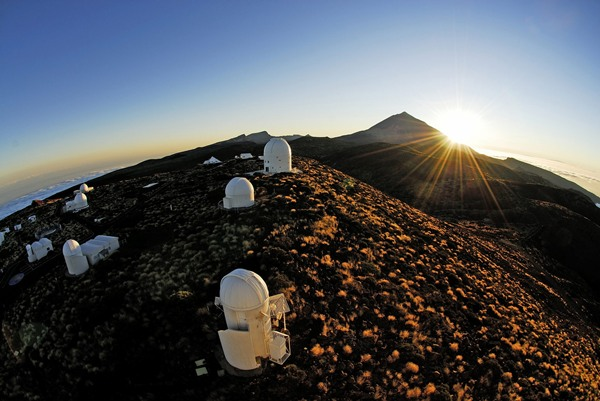
\includegraphics[width=0.7\linewidth]{FIGURES/IAC}
		\end{center}
\end{frame}
%%%%%%%%%%%%%%%%%%%%%%%%%%%%%%%%%%%%%%%%%%%%%%%%%%%%%%%%%%%%%%

%%%%%%%%%%%%%%%%%%%%%%%%%%%%%%%%%%%%%%%%%%%%%%%%%%%%%%%%%%%%%%
\begin{frame}
    \frametitle{Gran Telescopio Canarias}
    \block{GTC}
    \endblock{}
		\begin{center}
    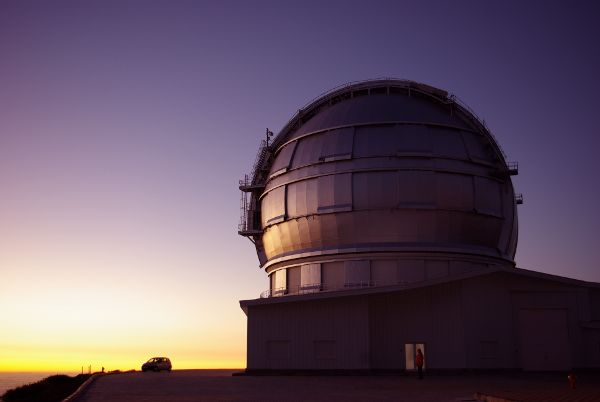
\includegraphics[width=0.8\linewidth]{FIGURES/GTC}
		\end{center}
\end{frame}
%%%%%%%%%%%%%%%%%%%%%%%%%%%%%%%%%%%%%%%%%%%%%%%%%%%%%%%%%%%%%%

%%%%%%%%%%%%%%%%%%%%%%%%%%%%%%%%%%%%%%%%%%%%%%%%%%%%%%%%%%%%%%
\begin{frame}
    \frametitle{Proyecto GOYA}
    \centering{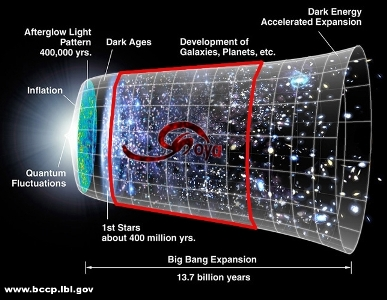
\includegraphics[width=0.4\linewidth]{FIGURES/goya}}
    \block{GOYA: Galaxy Origins and Young Assembly}
    \begin{itemize}
		\item Objetivo: entender cómo se forman y evolucionan las galaxias observando sus propiedades en una época de máximo crecimiento
		\item Investiga las propiedades de las galaxias más lejanas
		\item A distancias de 8000--13000 millones de años luz
		\item Llevará a cabo la primera exploración sistemática de la población de galaxias poco después del nacimiento del universo
    \end{itemize}
    \endblock{}
\end{frame}
%%%%%%%%%%%%%%%%%%%%%%%%%%%%%%%%%%%%%%%%%%%%%%%%%%%%%%%%%%%%%%

%%%%%%%%%%%%%%%%%%%%%%%%%%%%%%%%%%%%%%%%%%%%%%%%%%%%%%%%%%%%%%
\begin{frame}
    \frametitle{El Proyecto EMIR}
    \centering{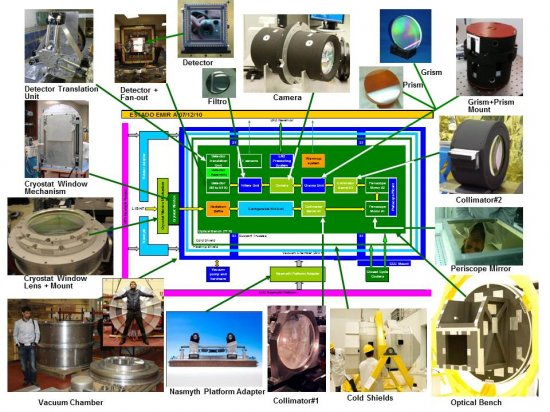
\includegraphics[width=0.7\linewidth]{FIGURES/emir}}
    %\centering{
\includegraphics[width=0.6\linewidth]{FIGURES/logoEMIR}}
    \block{EMIR: Espectrógrafo Multiobjeto Infrarrojo}
		EMIR es un cámara de gran campo y espectrógrafo de resolución intermedia en el infrarrojo cercano para el telescopio GTC
    \endblock{}
\end{frame}
%%%%%%%%%%%%%%%%%%%%%%%%%%%%%%%%%%%%%%%%%%%%%%%%%%%%%%%%%%%%%%

%\begin{frame}{Índice}
% \begin{columns}[t]
%		\column{.5\linewidth}
%		  \alert<1>{\small{\tableofcontents[sections={1}]}}
%		  \vspace{5mm}
%		  \alert<2>{\small{\tableofcontents[sections={2}]}}
%		  \vspace{5mm}
%		  \alert<3>{\small{\tableofcontents[sections={3}]}}
%		  \vspace{5mm}
%      \alert<4>{\small{\tableofcontents[sections={4}]}}
%		  \vspace{5mm}
% \end{columns}
%\end{frame}


%%%%%%%%%%%%%%%%%%%%%%%%%%%%%%%%%%%%%%%%%%%%%%%%%%%%%%%%%%%%%
%%%%%%%%%%%%%%%%%%%%%%%%%%%%%%%%%%%%%%%%%%%%%%%%%%%%%%%%%%%%%
%%%%%%%%%%%%%%%%%%%%%%%%%%%%%%%%%%%%%%%%%%%%%%%%%%%%%%%%%%%%%

%\AtBeginSection[]
%{
%   \begin{frame}
%       \frametitle{Índice}
%       \footnotesize{
%         \tableofcontents[currentsection,hideothersubsections]
%       }
%   \end{frame}
%}
%
